\chapter{फूल, फल और बीज}\label{ch:g3:flowers-fruits-seeds}

अप्रैल में चेरी का \omterm{def:g1:plants-around-us:tree}{पेड़} फूलों से सफ़ेद रहता है; जून में उस पर चेरियाँ
लटकती हैं। \omterm{def:g3:flowers-fruits-seeds:parts}{फूल} कहाँ गए --- और \omterm{prop:g3:flowers-fruits-seeds:transform}{फल} कहाँ से आए? इसका उत्तर जीवित दुनिया के
सबसे सुंदर बदलावों में से एक है: \omterm{def:g3:flowers-fruits-seeds:parts}{फूल} ग़ायब नहीं होता, वह ख़ुद \omterm{prop:g3:flowers-fruits-seeds:transform}{फल}
\emph{बन जाता} है।

\section{फूल के भीतर झाँकना}

\begin{definition}[फूल के भाग]\label{def:g3:flowers-fruits-seeds:parts}
\emph{फूल}\index{फूल} \omterm{def:g1:plants-around-us:plant}{पौधे} का वह भाग है जो \omterm{def:g2:from-seed-to-plant:seed}{बीज} बनाएगा। बाहर से भीतर की
ओर:
\begin{enumerate}
  \item \emph{पंखुड़ियाँ}\index{पंखुड़ी}, रंगीन और महकती हुई, जो आने
        वाले \omterm{prop:g3:sorting-living-things:groups}{कीटों} को खींचती हैं;
  \item \emph{पुंकेसर}\index{पुंकेसर}, पतली डंडियाँ जिन पर
        \emph{पराग}\index{पराग} लगा रहता है, यानी महीन पीला चूर्ण;
  \item और ठीक बीच में \emph{स्त्रीकेसर}\index{स्त्रीकेसर}, एक छोटी
        सुराही; उसके भीतर गहराई में फूल के भावी \omterm{def:g2:from-seed-to-plant:seed}{बीज} पड़े रहते हैं।
\end{enumerate}
\end{definition}

\begin{omfigure}
\begin{tikzpicture}
  \node[anchor=south west, inner sep=0] (img) at (0,0)
    {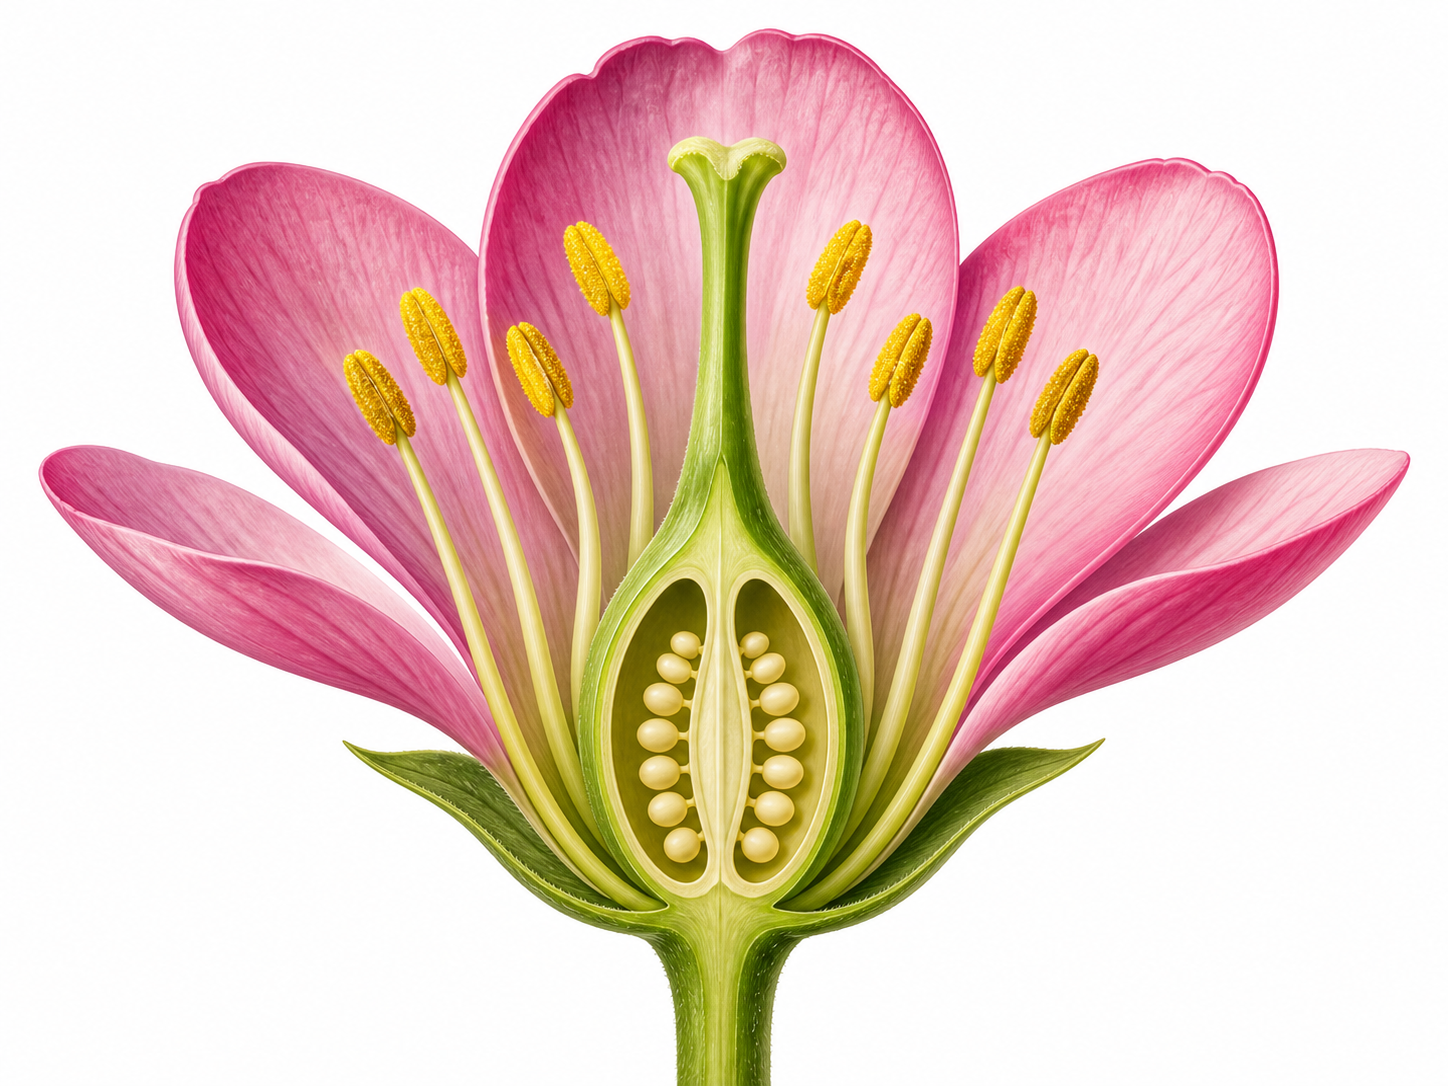
\includegraphics[width=0.6\linewidth]{images/book1/ai/fig-flower-cutaway.png}};
  \begin{scope}[x={(img.south east)}, y={(img.north west)},
      every node/.style={font=\small}]
    \draw[omDef, thick] (0.82,0.80) -- (0.93,0.90) node[above] {पंखुड़ी};
    \draw[omDef, thick] (0.72,0.68) -- (1.03,0.66)
      node[right, align=left] {पुंकेसर, जिस पर\\ पराग लगा है};
    \draw[omDef, thick] (0.56,0.36) -- (1.03,0.34)
      node[right, align=left] {स्त्रीकेसर: भावी बीज\\ इसी के भीतर हैं};
    \draw[omDef, thick] (0.505,0.05) -- (0.66,0.04) node[right] {डंठल};
  \end{scope}
\end{tikzpicture}

{\small बीच से कटा हुआ \omterm{def:g3:flowers-fruits-seeds:parts}{फूल}: चारों ओर \omterm{def:g3:flowers-fruits-seeds:parts}{पंखुड़ियाँ}, \omterm{def:g3:flowers-fruits-seeds:parts}{पराग} लिए \omterm{def:g3:flowers-fruits-seeds:parts}{पुंकेसर}, और
बीच में \omterm{def:g3:flowers-fruits-seeds:parts}{स्त्रीकेसर}, जिसके भीतर भावी \omterm{def:g2:from-seed-to-plant:seed}{बीज} हैं।}
\end{omfigure}

\begin{example}[ट्यूलिप का विच्छेदन]\label{ex:g3:flowers-fruits-seeds:tulip}
मुरझाते ट्यूलिप को धीरे-धीरे, \omterm{def:g3:flowers-fruits-seeds:parts}{पंखुड़ी} दर \omterm{def:g3:flowers-fruits-seeds:parts}{पंखुड़ी} खोलो। भीतर \omterm{def:g3:flowers-fruits-seeds:parts}{पुंकेसर} खड़े
मिलते हैं --- किसी एक को उँगली पर रगड़ो और वह पीली \omterm{def:g3:flowers-fruits-seeds:parts}{पराग} की धूल छोड़
जाता है --- और बीच में मोटा हरा \omterm{def:g3:flowers-fruits-seeds:parts}{स्त्रीकेसर}। \omterm{def:g3:flowers-fruits-seeds:parts}{स्त्रीकेसर} को आड़ा काटो
(यह काम किसी बड़े की छुरी से) और वे सामने हैं: नन्हे पीले भावी \omterm{def:g2:from-seed-to-plant:seed}{बीजों}
की क़तारें।
\end{example}

\section{फूल से फल तक}

\begin{proposition}[परागण, फिर बदलाव]\label{prop:g3:flowers-fruits-seeds:transform}
बदलाव शुरू होने के लिए \omterm{def:g3:flowers-fruits-seeds:parts}{पराग} का \omterm{def:g3:flowers-fruits-seeds:parts}{स्त्रीकेसर} तक पहुँचना ज़रूरी है --- यही
क़दम \emph{परागण}\index{परागण} है। ढोने का ज़्यादातर काम मधुमक्खियाँ
और दूसरे \omterm{prop:g3:sorting-living-things:groups}{कीट} करते हैं, जो \omterm{def:g3:flowers-fruits-seeds:parts}{फूल} दर \omterm{def:g3:flowers-fruits-seeds:parts}{फूल} रस पीते समय \omterm{def:g3:flowers-fruits-seeds:parts}{पराग} से सन जाते हैं;
कुछ काम हवा भी करती है। परागण के बाद:
\begin{itemize}
  \item \omterm{def:g3:flowers-fruits-seeds:parts}{पंखुड़ियाँ} और \omterm{def:g3:flowers-fruits-seeds:parts}{पुंकेसर}, अपना काम पूरा करके, मुरझाकर गिर जाते
        हैं;
  \item \omterm{def:g3:flowers-fruits-seeds:parts}{स्त्रीकेसर} फूलकर \emph{फल}\index{फल} बन जाता है;
  \item उसके भीतर के भावी \omterm{def:g2:from-seed-to-plant:seed}{बीज} \emph{बीज}\index{बीज} बन जाते हैं।
\end{itemize}
\omterm{prop:g3:flowers-fruits-seeds:transform}{फल} एक बदला हुआ \omterm{def:g3:flowers-fruits-seeds:parts}{स्त्रीकेसर} है, और हर सच्चा \omterm{prop:g3:flowers-fruits-seeds:transform}{फल} \omterm{def:g2:from-seed-to-plant:seed}{बीज} लिए रहता है।
\end{proposition}
\admitted

\begin{example}[एक चेरी को बनते देखना]\label{ex:g3:flowers-fruits-seeds:cherry}
चेरी के एक ही \omterm{def:g3:flowers-fruits-seeds:parts}{फूल} का पीछा करो। अप्रैल: सफ़ेद \omterm{def:g3:flowers-fruits-seeds:parts}{पंखुड़ियाँ}, भिनभिनाती
मधुमक्खियाँ। मई: \omterm{def:g3:flowers-fruits-seeds:parts}{पंखुड़ियाँ} बर्फ़ की तरह गिरतीं; जहाँ हर \omterm{def:g3:flowers-fruits-seeds:parts}{फूल} खड़ा था
वहाँ एक नन्ही हरी गोली --- यानी फूलता \omterm{def:g3:flowers-fruits-seeds:parts}{स्त्रीकेसर}। जून: वही गोली लाल
और मीठी हो चुकी --- एक चेरी, जिसके भीतर गुठली (उसका \omterm{def:g2:from-seed-to-plant:seed}{बीज}) है। \omterm{def:g3:flowers-fruits-seeds:parts}{फूल} गिरा
नहीं; सिर्फ़ उसकी \omterm{def:g3:flowers-fruits-seeds:parts}{पंखुड़ियाँ} गिरीं।
\end{example}

\begin{remark}[मधुमक्खियाँ नहीं, तो चेरियाँ नहीं]\label{rem:g3:flowers-fruits-seeds:bees}
चेरी उगाने वाले मधुमक्खी-पालकों के छत्तों का अपने बाग़ों में स्वागत
करते हैं --- \omterm{prop:g3:sorting-living-things:groups}{कीटों} के आए बिना ज़्यादातर \omterm{def:g3:flowers-fruits-seeds:parts}{फूल} बिना परागण के रह जाते और
\omterm{prop:g3:flowers-fruits-seeds:transform}{फल} बने बिना ही गिर जाते। मधुमक्खी \omterm{def:g3:flowers-fruits-seeds:parts}{फूल} से चोरी नहीं कर रही; \omterm{def:g3:flowers-fruits-seeds:parts}{फूल} और
मधुमक्खी एक-दूसरे का पोषण करते हैं: मधुमक्खी को रस, और \omterm{def:g1:plants-around-us:plant}{पौधे} को \omterm{def:g3:flowers-fruits-seeds:parts}{पराग} की
ढुलाई।
\end{remark}

\begin{omfigure}
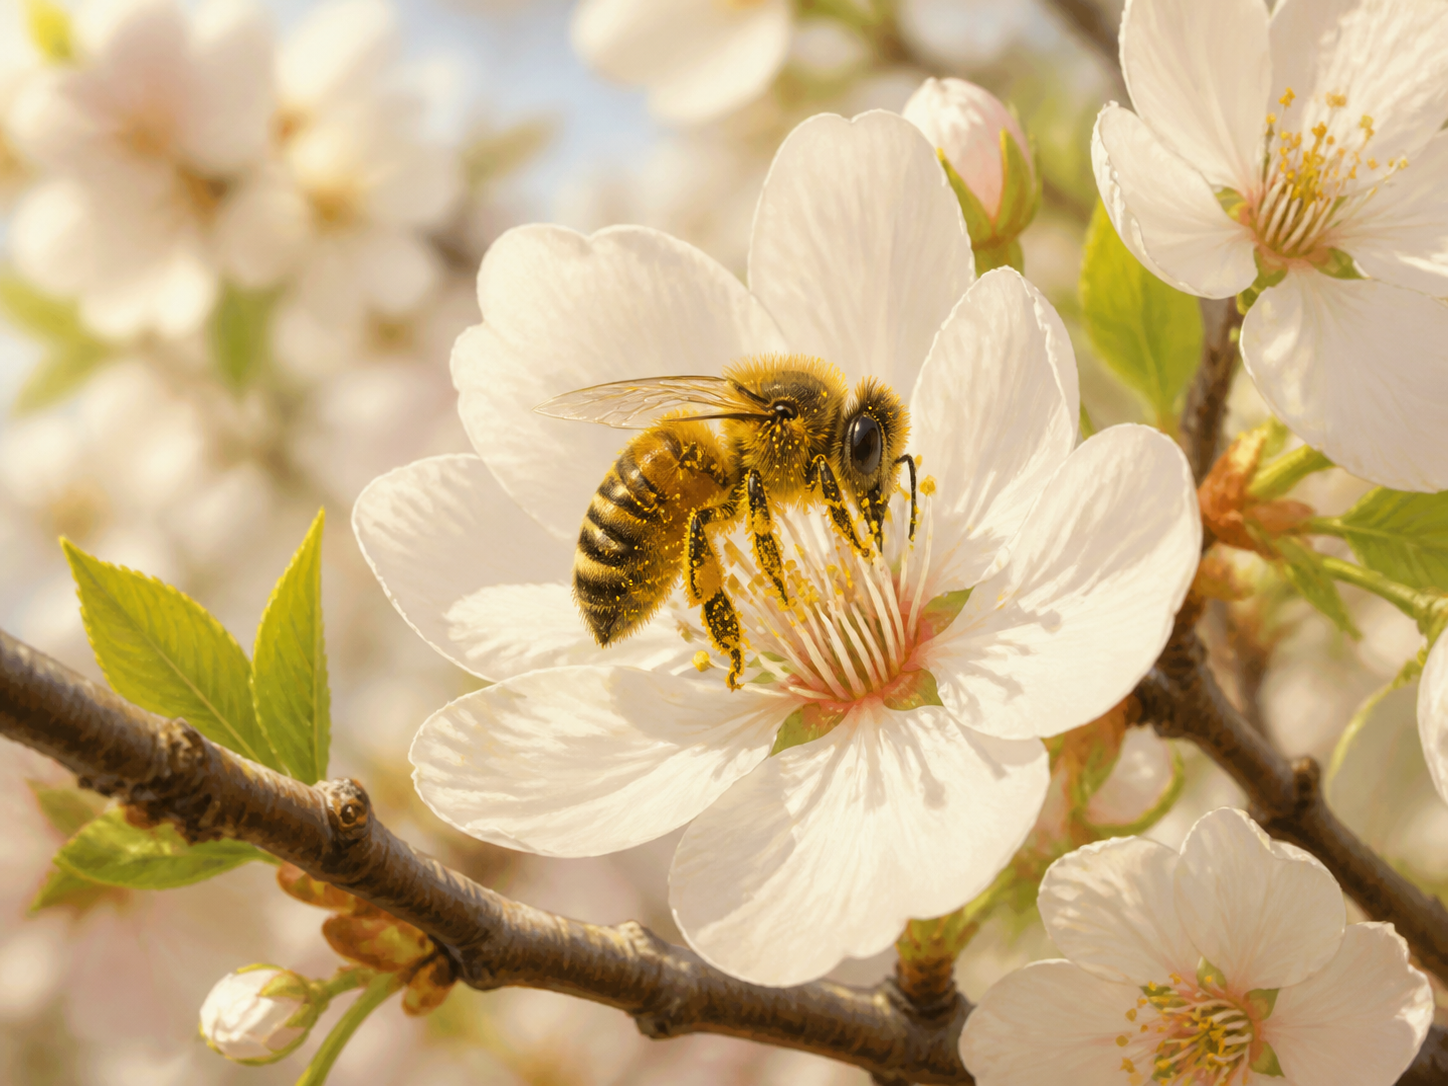
\includegraphics[width=0.58\linewidth]{images/book1/ai/g3-flowers-bee.png}

{\small परागण होते हुए: चेरी के \omterm{def:g3:flowers-fruits-seeds:parts}{फूल} में गहरे धँसी एक मधुमक्खी, उस \omterm{def:g3:flowers-fruits-seeds:parts}{पराग}
से सनी हुई जो वह अगले \omterm{def:g3:flowers-fruits-seeds:parts}{फूल} तक पहुँचाएगी।}
\end{omfigure}

\section{फल या फल नहीं?}

\begin{method}[बीज की जाँच]\label{met:g3:flowers-fruits-seeds:test}
सब्ज़ी वाले की कोई चीज़ जीवविज्ञानी के अर्थ में \omterm{prop:g3:flowers-fruits-seeds:transform}{फल} है या नहीं, यह तय
करने के लिए:
\begin{enumerate}
  \item उसे काटो;
  \item \omterm{def:g2:from-seed-to-plant:seed}{बीज} ढूँढ़ो (या गुठली, जो सख़्त \omterm{def:g1:animals-around-us:covering}{खोल} में बंद एक \omterm{def:g2:from-seed-to-plant:seed}{बीज} है);
  \item भीतर \omterm{def:g2:from-seed-to-plant:seed}{बीज} हैं --- तो वह किसी \omterm{def:g3:flowers-fruits-seeds:parts}{फूल} के \omterm{def:g3:flowers-fruits-seeds:parts}{स्त्रीकेसर} से बना है: यानी
        \omterm{prop:g3:flowers-fruits-seeds:transform}{फल}। कहीं \omterm{def:g2:from-seed-to-plant:seed}{बीज} नहीं --- तो वह \omterm{def:g1:plants-around-us:plant}{पौधे} का कोई और भाग है: \omterm{def:g1:plants-around-us:parts}{जड़}, \omterm{def:g1:plants-around-us:parts}{डंठल}
        या \omterm{def:g1:plants-around-us:parts}{पत्ती}।
\end{enumerate}
\end{method}

\begin{example}[सब्ज़ी वाले के यहाँ चौंकाने वाली बातें]\label{ex:g3:flowers-fruits-seeds:surprise}
\omterm{def:g2:from-seed-to-plant:seed}{बीज} की जाँच चौंका देती है। टमाटर: \omterm{def:g2:from-seed-to-plant:seed}{बीजों} से भरा --- यानी \omterm{prop:g3:flowers-fruits-seeds:transform}{फल}, सलाद का
कटोरा चाहे जो कहे। खीरा और तोरी: \omterm{def:g2:from-seed-to-plant:seed}{बीज} --- \omterm{prop:g3:flowers-fruits-seeds:transform}{फल}। हरी फली: क़तार में \omterm{def:g2:from-seed-to-plant:seed}{बीज} ---
\omterm{prop:g3:flowers-fruits-seeds:transform}{फल}। गाजर: कोई \omterm{def:g2:from-seed-to-plant:seed}{बीज} नहीं --- \omterm{def:g1:plants-around-us:parts}{जड़} (\cref{exo:g1:plants-around-us:10} ने
इसे बूझ लिया था)। सलाद-पत्ता: कोई \omterm{def:g2:from-seed-to-plant:seed}{बीज} नहीं --- \omterm{def:g1:plants-around-us:parts}{पत्तियाँ}। आलू: कोई \omterm{def:g2:from-seed-to-plant:seed}{बीज}
नहीं --- ज़मीन के नीचे फूला हुआ \omterm{def:g1:plants-around-us:parts}{डंठल}।
\end{example}

\begin{remark}[रसोई के शब्द, विज्ञान के शब्द]\label{rem:g3:flowers-fruits-seeds:words}
रसोई में ``\omterm{prop:g3:flowers-fruits-seeds:transform}{फल}'' का मतलब मीठा है और ``सब्ज़ी'' का नमकीन --- मिठाई की
योजना बनाने के लिए काम का, \omterm{def:g1:living-or-not:living}{जीवविज्ञान} के लिए बेकार। जीवविज्ञानी का
शब्द \omterm{def:g2:from-seed-to-plant:seed}{बीज} की जाँच के पीछे चलता है। दोनों शब्दावलियाँ ठीक हैं, बशर्ते
तुम्हें पता हो कि तुम कौन-सी बोल रहे हो।
\end{remark}

\section{अभ्यास}

\begin{exercise}[$\star$]\label{exo:g3:flowers-fruits-seeds:1}
\omterm{def:g3:flowers-fruits-seeds:parts}{फूल} के भागों के नाम बाहर से भीतर की ओर बताओ, और हर भाग का काम भी।
\end{exercise}

\begin{exercise}[$\star$]\label{exo:g3:flowers-fruits-seeds:2}
\omterm{def:g3:flowers-fruits-seeds:parts}{पराग} क्या है, और वह कहाँ मिलता है? परागण क्या है?
\end{exercise}

\begin{exercise}[$\star$]\label{exo:g3:flowers-fruits-seeds:3}
परागण के बाद क्या होता है: (क) \omterm{def:g3:flowers-fruits-seeds:parts}{पंखुड़ियों} का? (ख) \omterm{def:g3:flowers-fruits-seeds:parts}{स्त्रीकेसर} का? (ग)
उसके भीतर के भावी \omterm{def:g2:from-seed-to-plant:seed}{बीजों} का?
\end{exercise}

\begin{exercise}[$\star$]\label{exo:g3:flowers-fruits-seeds:4}
सफ़ेद \omterm{def:g3:flowers-fruits-seeds:parts}{फूल} से लाल \omterm{prop:g3:flowers-fruits-seeds:transform}{फल} तक एक चेरी की कहानी तारीख़ वाले तीन क़दमों में
दोहराओ।
\end{exercise}

\begin{exercise}[$\star$]\label{exo:g3:flowers-fruits-seeds:5}
चेरी उगाने वाले बाग़ में मधुमक्खियों के छत्तों का स्वागत क्यों करते हैं?
\end{exercise}

\begin{exercise}[$\star$]\label{exo:g3:flowers-fruits-seeds:6}
\omterm{def:g2:from-seed-to-plant:seed}{बीज} की जाँच बताओ, और उसे टमाटर तथा गाजर पर लगाओ।
\end{exercise}

\begin{exercise}[$\star$]\label{exo:g3:flowers-fruits-seeds:7}
\omterm{def:g2:from-seed-to-plant:seed}{बीज} की जाँच से बताओ कि ये \omterm{prop:g3:flowers-fruits-seeds:transform}{फल} हैं या नहीं: खीरा, सलाद-पत्ता, हरी फली,
आलू?
\end{exercise}

\begin{exercise}[$\star$]\label{exo:g3:flowers-fruits-seeds:8}
करके देखो: घर पर रसोई की तीन चीज़ें काटो और हर एक पर \omterm{def:g2:from-seed-to-plant:seed}{बीज} की जाँच चलाओ।
किसने तुम्हें चौंकाया?
\end{exercise}

\begin{exercise}[$\star\star$]\label{exo:g3:flowers-fruits-seeds:9}
अप्रैल में देर से पड़े पाले से आलूबुख़ारे के \omterm{def:g1:plants-around-us:tree}{पेड़} के सारे \omterm{def:g3:flowers-fruits-seeds:parts}{फूल} मर जाते
हैं। जून की फ़सल कैसी होगी, और क्यों?
\cref{prop:g3:flowers-fruits-seeds:transform} का इस्तेमाल करो।
\end{exercise}

\begin{exercise}[$\star\star$]\label{exo:g3:flowers-fruits-seeds:10}
``सेब इसलिए उगता है कि हमें खाने को कुछ अच्छा मिले।'' सेब के \omterm{def:g1:plants-around-us:tree}{पेड़} की
नज़र से सेब असल में किसलिए है? उसके बीचोंबीच क्या है, और उनमें से हर
एक क्या बन सकता है? (\cref{ch:g2:from-seed-to-plant} याद करो।)
\end{exercise}
